\documentclass[11pt]{article}
\usepackage[margin=0.8in]{geometry}
\usepackage{graphicx}
\usepackage{longtable}
\usepackage[T1]{fontenc}
\usepackage{hyperref}
\title{Current formal target provenance inventory}
\author{Static evidence review}
\date{25 October 2026}
\begin{document}
\maketitle
\noindent\textbf{Named main:} \texttt{0b38ac1157f777cb4a77d35e53d7ed583c541eb4}.\\
\textbf{Formal tree:} \texttt{96f334e856c87d397b5db720899d833a75db0352}.\\
\textbf{Scope:} Repository blob and declared-path inventory only. This is no theorem build, experimental replay, or semantic sign-off.

\section*{Observations}
\begin{longtable}{lr}
Target YAML specs & 87\\
Existing referenced theorem paths & 87\\
Distinct declared source paths & 30\\
Specs with canonical EXP identifier & 12\\
Source paths under experiments/ & 6\\
Direct /runs/ source paths & 0\\
Specs with explicit run reference & 0\\
\end{longtable}
The canonical IDs in those twelve specs are \texttt{EXP-BINSTD-8bdf86} and \texttt{EXP-FROB-91ee9c}. Source status labels are COMPUTED (54), PROVED (23), STATED (8), DERIVATION (1), and MEASURED WITH ALGEBRAIC EXPLANATION (1). These labels are not independently checked outcomes.

\begin{center}
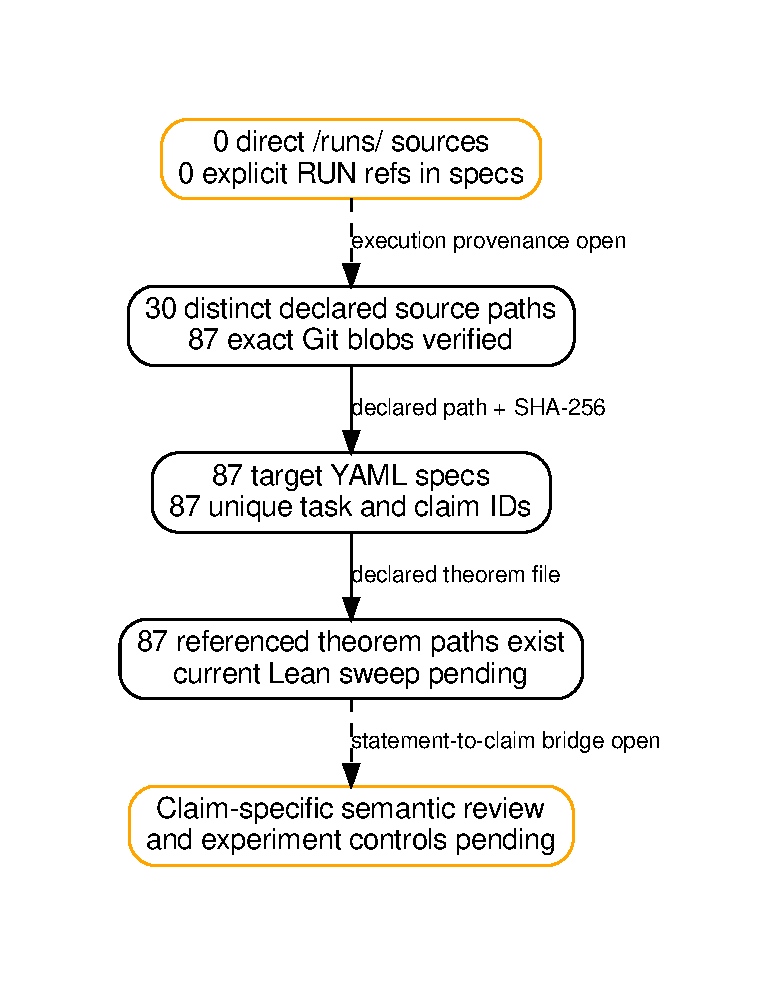
\includegraphics[height=0.30\textheight,keepaspectratio]{coverage.pdf}
\end{center}
\noindent\small{Solid links represent declared repository paths. Dashed links mark open execution provenance and statement-to-claim obligations. Counts describe the named commit only.}

\section*{Interpretation and next check}
The archived full per-target sweep covered 84 targets on an earlier tree; the current set has 87. Three later targets have separate exact-source receipts, but no fresh full 87-target sweep or independent semantic review across all claims is established. File existence cannot prove compilation or that a theorem matches a historical experiment. Absence of a direct run path does not prove that no other provenance exists. Generic theorems may legitimately lack experiment IDs.

Before a claim is promoted, review its frozen source and run evidence, precise theorem hypotheses, model bridge, controls, and independent semantic assessment. Empirical measurements require provenance and uncertainty checks even when no theorem is suitable. No quantitative performance or attack-cost claim is made here. The open repository problem is \texttt{problems/formal-target-semantic-fidelity-unreviewed.md}. Existing scientific graphs and measured dashboards are unchanged because no new result or decision was recorded.

\end{document}
